\section{Task 8 - Admin}
\subsection{The task}
The admin (with defined credentials admin, password nimda) should be redirected from the main page to an admin page where he can see the current logged users and their points.

If a normal user tries to access the page, it returns error code 401. (Note: the correct code to return should be 403 Forbidden and not 401 Unauthorized, but we will follow the assignment request).
\subsection{Sessions in the Context}
Since we do not have a native method to get all the current sessions of our system, we need to save them in the servlet context each time a session is created (login or registration) or updated (points given at the end of a game).

Since the context is shared memory, all the functions that modify it should be in a synchronized block.
\subsubsection{Create or update Session}
A new session creation is done by the function \textit{Login.setSession()}. Here, we get the context, add the new session and update it. If the session already has an username, it means that the user is doing another login, so we update the session username value. At the same time, we search the context for the old session and delete it, before adding a new one. In this way, we do not have multiple open sessions in the context for an user that changes credentials. (Note: for this reason, during testing accessing first as an user and then as an admin deletes the first session and the admin page would only show the admin as online. It is needed to log in as the user from another browser or from a private/incognito page, which uses different sessions).

A session update is also done by the game page to update the points. In this case, we search in the context for the user session and update the points there too.
\subsubsection{SessionListener.java}
If a session ends, we need to remove it from the context. This can be done with an \textit{HttpSessionListener}. We can implement it with the class \textit{SessionListener.java}, where we simply search for the expired session username and delete it from the context.


\subsection{Admin page}
\subsubsection{admin.jsp}
The admin jsp page takes as an argument the list of users to show. It contains a simple table with three columns: rank, username and points. The reason for the rank column is that we set up the list of users to be ordered, but this was not required.

This page does not redirect if a simple user tries to access the file directly instead of passing first by the java class. It is not a problem, however, since the page itself does not have the capability to access the context and gather the sensitive data.
\subsubsection{unauthorized.jsp}
This page simply shows an error message and a link to return to the main page.
\subsubsection{Admin.java}
If the user is not authenticated, redirects to the main page with the static method \textit{Main.getUserSession}. 

If the username is not the admin one (set up by a static variable \textit{ADMIN\_USERNAME} because needed also by \textit{Main.java}), it redirects to \textit{unauthorized.jsp}. 

If the user is the admin, it gets all the session saved in the context, sort them and forward them to \textit{admin.jsp}


\subsubsection{Screenshots}
\begin{figure}[H]
  \centering
  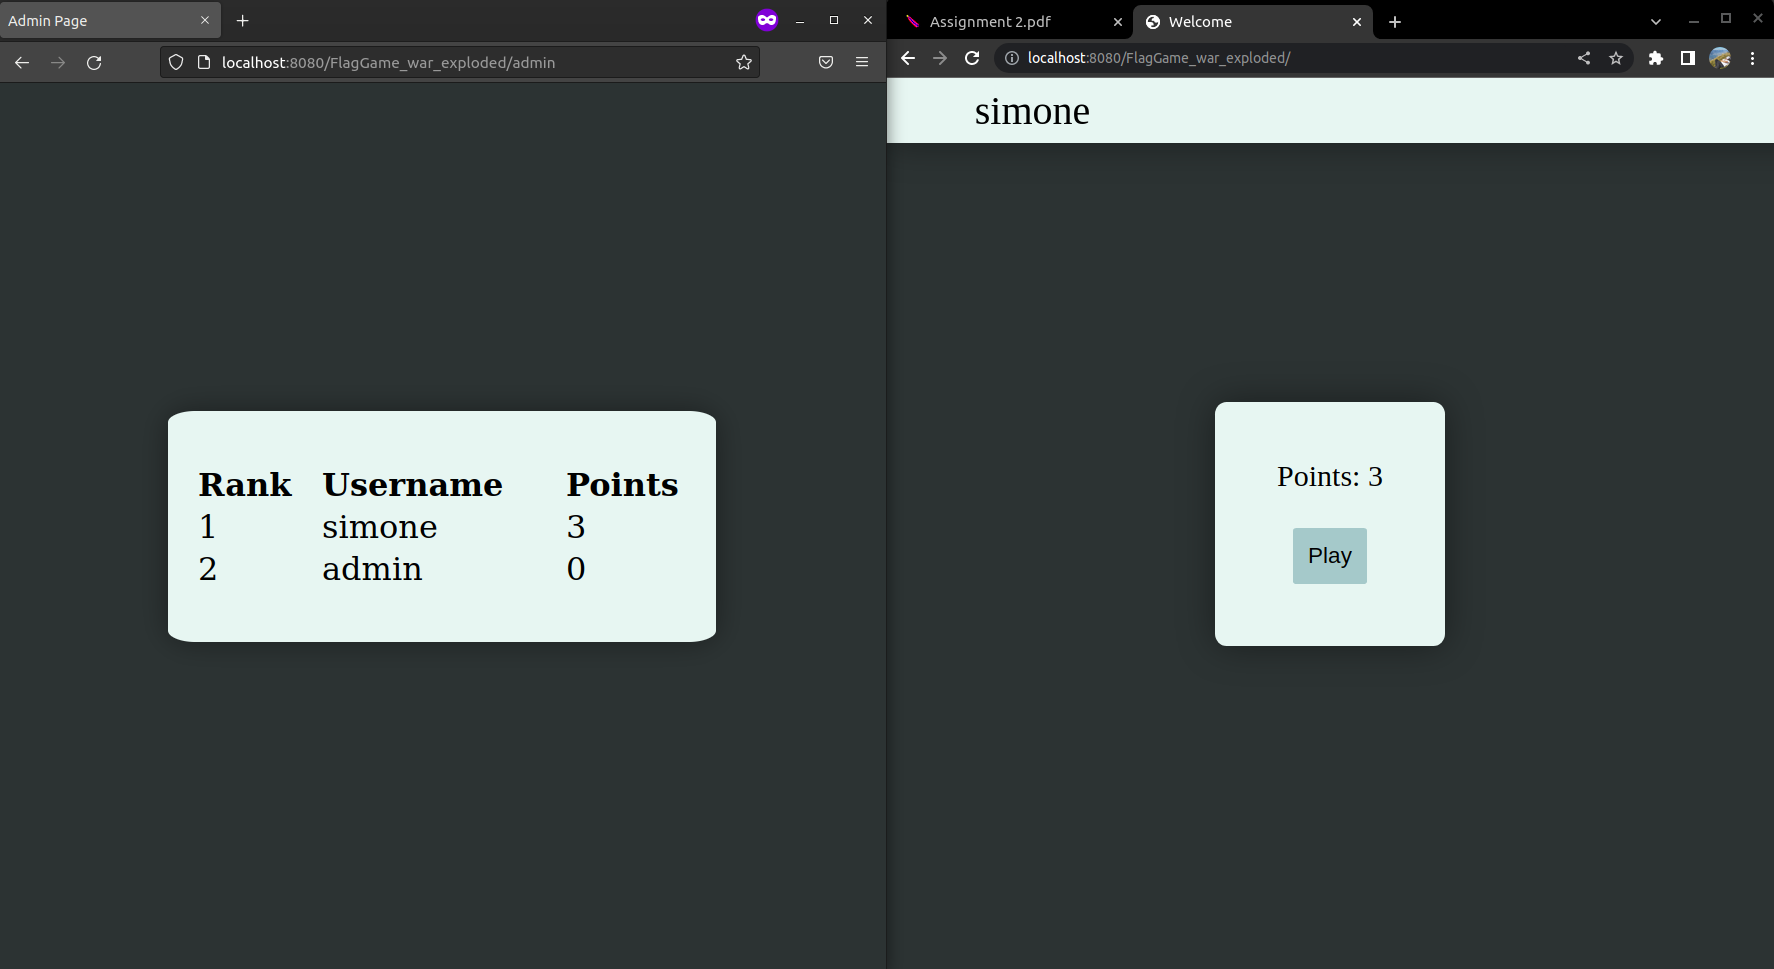
\includegraphics[width=\columnwidth]{admin.png}
  \caption{Admin page and an user main page}
\end{figure}
\begin{figure}[H]
  \centering
  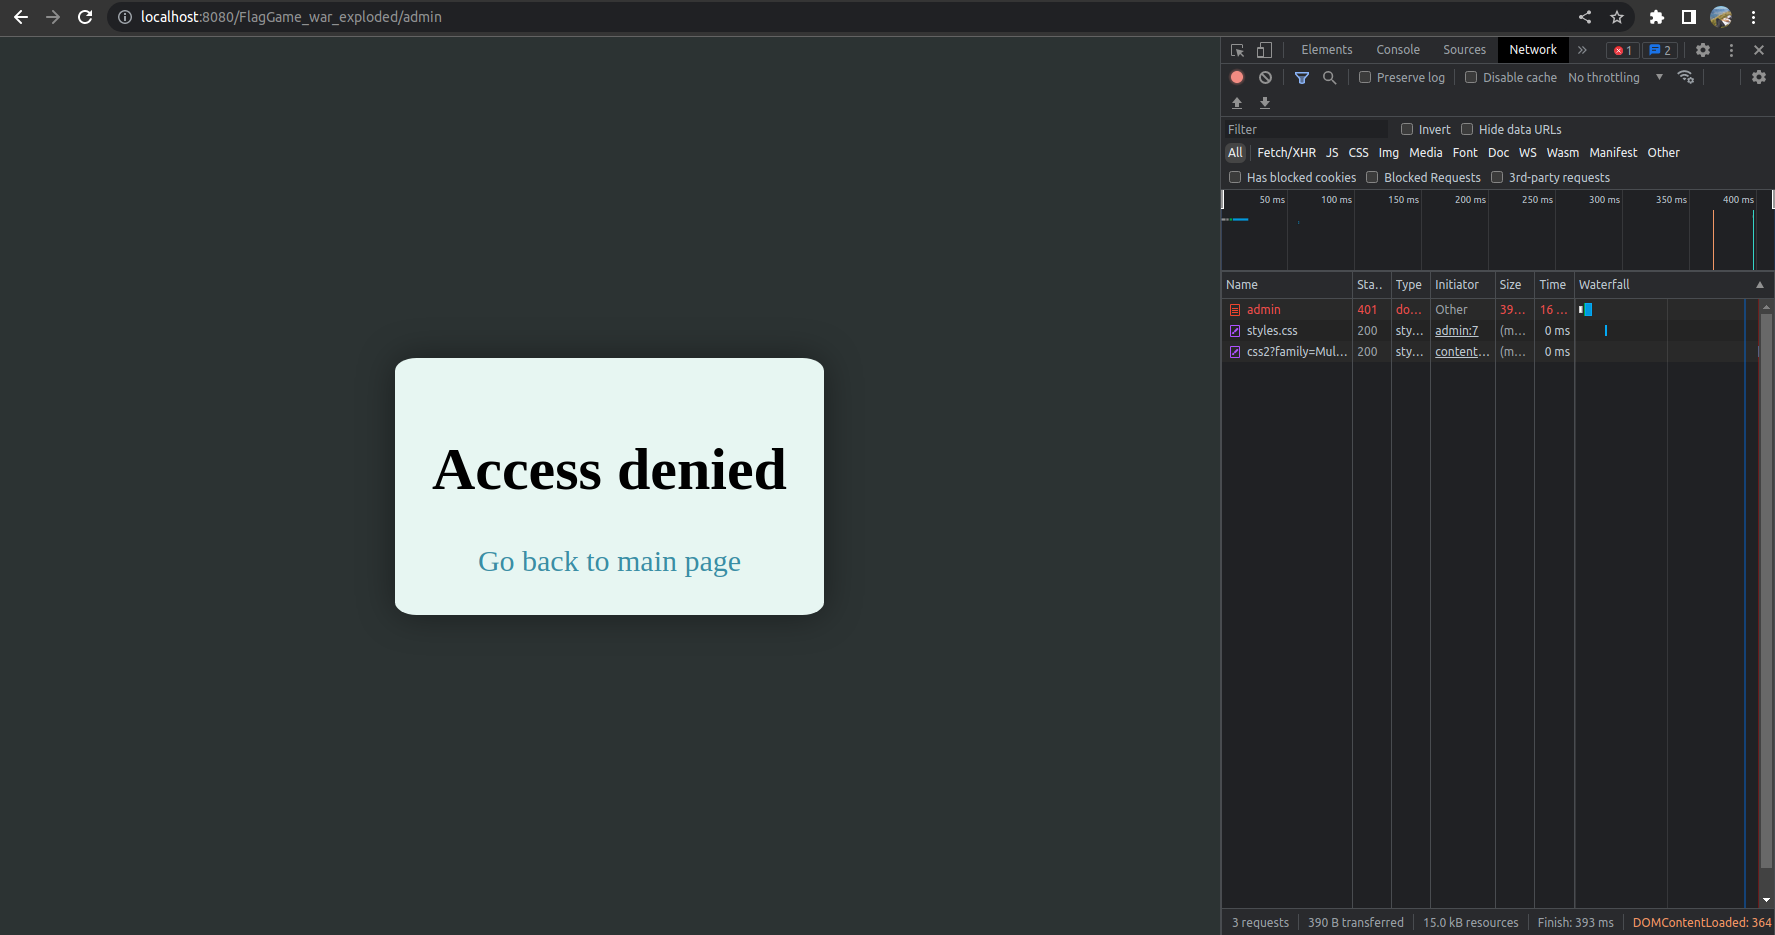
\includegraphics[width=\columnwidth]{unauthorized.png}
  \caption{Unauthorized page. The status code is 401}
\end{figure}